\contribution{The Control Status Registers}
\shortcontributor{CS6230 : CAD for VLSI Project Report}
\shortcontribution{Vector Extensions}
\headnum{6}
\begin{paper}
\renewcommand*{\pagemark}{}
\section*{}
The Control Status Registers (CSRs) is the only communication path between the processor and the accelerator. There are multiple CSRs, each for a specific purpose. Each CSR has an exclusive address, as indicated in the figure given below. When the CPU encounters a vector instruction, it writes the required operands, i.e., the address of the source, block size of the vector, the Opcode, and the address where the result is to be stored into the CSRs. After these operands are written, the CPU writes one into the Start flag. This action causes the accelerator to start its operation. The Aux CSR is used for any extra data required by any new functionality. This design helps in adding functionality without significantly altering the design. For instance, the pointer to the minima index in vector neg operation utilizes the Aux register.\\
\begin{figure}[H]
\centering
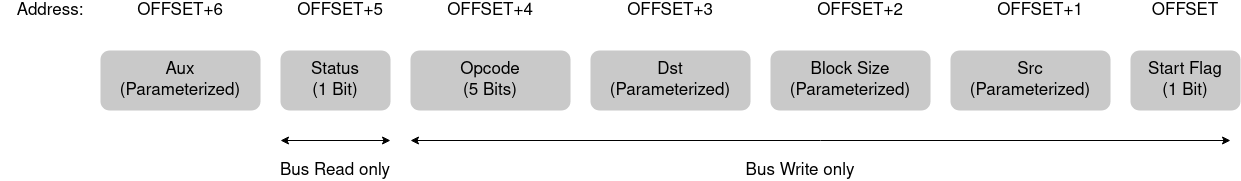
\includegraphics[width=\textwidth]{Images/VectorExtensions-CSRUniary(1).png}
\caption{\content Control status Registers for a Unary Vector Extension.}
\end{figure}

\noindent There is also a 1-Bit status register, which, when equals one, means that the accelerator has completed its operation and is idle.
\section*{Interface with the Bus\sdot}
The CSRs interface the Bus through a BusSlave. This means that CSRs cannot launch a request by themselves. The CSR's can only respond to read/write requests initiated by the processor or any other masters. So the CPU must periodically ping the accelerator to know the status of any operation previously initiated. The \textttt{Start Flag, Src, Block Size, Dst, and Opcode} are write-only. A null response is returned if the CPU attempts to read them. Similarly, the CPU can only read the \texttt{Status} register. Any attempts to write is ignored.

\end{paper}